% fig-store.tex: a store with the head, as a sequence diagram (draft of 5 Nov 2026, from Figure 4.1 of the thesis).
% Build from this folder:  pdflatex fig-store.tex     The blue arrows are the two requests this thesis adds.
% Simplified on purpose: the receipt file and the check of the local copy's version are in the text of section 4.4.
\documentclass[tikz,border=4pt,11pt]{standalone}
% style.tex: what the four diagrams share (colours, fonts, the look of a party, a message, a note).
% The one accent colour is the blue of the latency charts; it always means "the head", the thing this thesis adds.
% Everything else is black or grey, so the figures still read when printed in black and white.
\usepackage[T1]{fontenc}
\usepackage{mathptmx}
\usetikzlibrary{positioning,calc,arrows,fit,backgrounds}
\definecolor{head}{HTML}{2A78D6}
\definecolor{ink}{HTML}{0B0B0B}
\definecolor{inktwo}{HTML}{52514E}
\definecolor{soft}{HTML}{F0EFEC}
\definecolor{rule}{HTML}{C3C2B7}
\tikzset{
  every picture/.style={font=\small, >=latex},
  party/.style={draw=ink, fill=soft, rounded corners=2pt, minimum width=3.4cm, minimum height=0.8cm, align=center, font=\small\bfseries},
  box/.style={draw=ink, fill=soft, rounded corners=2pt, minimum width=3.9cm, minimum height=1.9cm, align=center},
  quiet/.style={draw=rule, text=inktwo},
  life/.style={draw=rule, line width=0.9pt},
  msg/.style={->, draw=ink, line width=0.7pt},
  rep/.style={->, draw=ink, line width=0.7pt, dashed},
  hmsg/.style={->, draw=head, line width=1.2pt},
  hrep/.style={->, draw=head, line width=1.2pt, dashed},
  bad/.style={->, draw=ink, line width=1.2pt, dashed},
  lab/.style={font=\footnotesize, inner sep=3pt, text=ink},
  act/.style={font=\footnotesize, align=left, text=ink, fill=white, draw=rule, rounded corners=1.5pt, inner sep=3pt},
  outcome/.style={font=\footnotesize, align=center, text=ink, fill=white, draw=ink, rounded corners=1.5pt, inner sep=4pt},
  side/.style={font=\footnotesize\itshape, align=left, text=inktwo},
  band/.style={fill=soft, draw=rule, rounded corners=2pt, minimum height=0.7cm, font=\footnotesize, text=inktwo},
  holds/.style={font=\footnotesize, text=inktwo, fill=white, draw=rule, rounded corners=1.5pt, inner sep=2.5pt},
}

\begin{document}
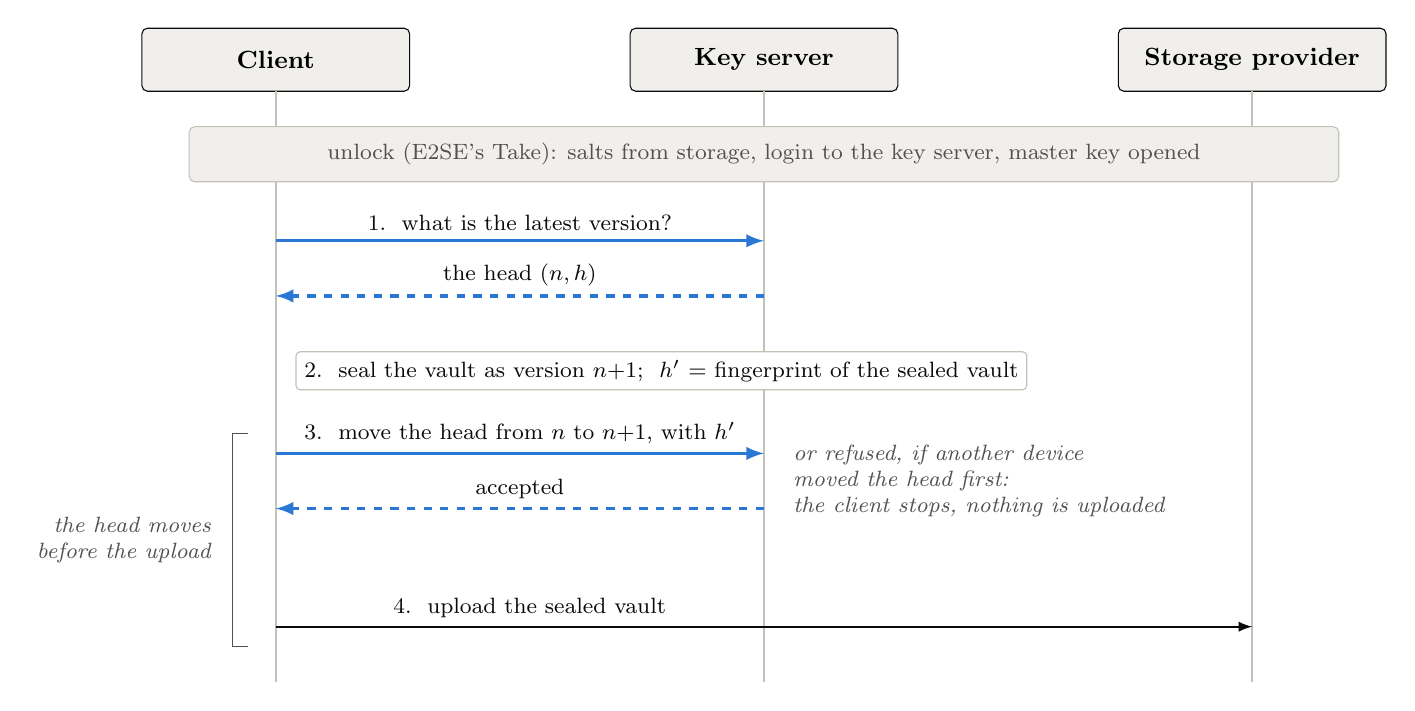
\begin{tikzpicture}
% the three parties and their lifelines
\node[party] (C) at (0,0)    {Client};
\node[party] (K) at (6.2,0)  {Key server};
\node[party] (D) at (12.4,0) {Storage provider};
\foreach \x in {0,6.2,12.4} \draw[life] (\x,-0.4) -- (\x,-7.9);
% unlock, E2SE's own procedure
\node[band, minimum width=14.6cm] at (6.2,-1.2) {unlock (E2SE's Take): salts from storage, login to the key server, master key opened};
% 1. fetch the head
\draw[hmsg] (0,-2.3) -- node[lab, above] {1.\ \ what is the latest version?} (6.2,-2.3);
\draw[hrep] (6.2,-3.0) -- node[lab, above] {the head $(n, h)$} (0,-3.0);
% 2. seal
\node[act, anchor=west] at (0.25,-3.95) {2.\ \ seal the vault as version $n{+}1$;\ \ $h'$ = fingerprint of the sealed vault};
% 3. reserve
\draw[hmsg] (0,-5.0) -- node[lab, above] {3.\ \ move the head from $n$ to $n{+}1$, with $h'$} (6.2,-5.0);
\draw[hrep] (6.2,-5.7) -- node[lab, above] {accepted} (0,-5.7);
\node[side, anchor=west] at (6.45,-5.35) {or refused, if another device\\ moved the head first:\\ the client stops, nothing is uploaded};
% 4. upload
\draw[msg] (0,-7.2) -- node[lab, above, pos=0.26] {4.\ \ upload the sealed vault} (12.4,-7.2);
% the ordering that matters
\draw[draw=inktwo, line width=0.5pt] (-0.35,-4.75) -- (-0.55,-4.75) -- (-0.55,-7.45) -- (-0.35,-7.45);
\node[side, anchor=east, align=right] at (-0.7,-6.1) {the head moves\\ before the upload};
\end{tikzpicture}
\end{document}
